\subsection{Motivation}

The paradigmatic problem of Fast Multipole Methods (\textbf{\gls{FMM}})
\footnote{The first usage of a technical term or abbreviation listed in the
glossary is highlighted throughout the text for ease of reference.} is the so
called $N$-Body problem. This classic problem refers to the calculation of the pairwise
interactions between $N$ particles over a potentially long-range, for example in
gravitational or electrostatic systems. The straightforward calculation can be
written in the form of the following sum,

\begin{equation}
\Phi(x_j) = \sum_{i=1}^N w_i K(x_i, x_j)
\label{eq:n_body_problem}
\end{equation}

Where $i, j \in [1,N]$ and $K(x, y)$ is called the Green's function, or equivalently
a `kernel function', where we are generally concerned with coordinates of particles in an
$n=2 \> \> \text{or} \> \> 3$ dimensional Hilbert space taking  $\{(x, y) | \> x, y \in \mathbb{R}^n \}$.
Additionally, each summand is weighted by $w_i$. For calculating electrostatic
problems in three dimensions, which is used as a model problem throughout this thesis, this goes to,

\begin{equation}
\Phi(x_j) = \sum_{i=1}^N q_iK(x_i, x_j)
\label{eq:electrostatic_paradigm}
\end{equation}

where $q_i$ refers to a charge density with the kernel function,

\begin{equation}
    K(x, y) = \frac{1}{4\pi \epsilon_0}\frac{1}{| x - y |}
\label{eq:laplace_kernel}
\end{equation}

the constant $\epsilon_0$ is the permittivity of free space. It's easy to see
how a naive direct application of this equation over $N$ particles
results in an algorithm of $O(N^2)$ complexity, therefore it's only practicable
for systems of moderate size. In realistic systems, we may be interested in
interactions involving $10^{6}$ to $10^8$ particles, making it impossible to
directly compute all interactions.

The analytic \gls{FMM} represented a sea change for $N$-Body simulation as it manages to
trade off computations for error to achieve an asymptotic complexity of just $O(N)$.
First presented by Greengard \cite{Greengard:1987:Yale}, the analytic \gls{FMM} comes
equipped with rigorous error bounds, making accurate massive $N$-Body simulations
feasible on available computing hardware.

The original analytic FMM developed by Greengard, solves the electrostatic problem
in two and three dimensions, this is equivalently known as the Poisson problem,
represented by the differential equation,

\begin{equation}
    \nabla^2 \phi =f
\label{eq:poisson}
\end{equation}

Where $\phi$ is some scalar potential to be determined, and $f$ is a scalar source
term which is usually known. For electrostatics the corresponding formulation
can be derived from Gauss' law as \cite{Griffiths:2017:CUP},

\begin{equation}
  \nabla^2 \phi = - \frac{q}{\epsilon_0}
\label{eq:electrostatic_poisson}
\end{equation}

where $\phi$ is the electrostatic potential, $q$ is the charge density and
$\epsilon_0$ is the permittivity of free space. It can therefore be seen that
the \gls{FMM} is actually solving the Poisson problem by formulating it as an
integral equation. The ubiquity of problems of the form (\ref{eq:n_body_problem})
in computational science has lead to diverse application of the FMM. For example,
in the modeling the electrostatic interactions of charged particles in complex
biological molecules at biologically relevant length scales \cite{Board:1992:CPL}.
The extension of FMMs to Helmholtz equations \cite{Rokhlin:1990:JCP}, has lead
to even more applications, such as in seismic and acoustic scattering
\cite{Hwu:2011:MKP}. Though as the focus of this thesis is on solving the Laplace
model problem for electrostatics, we mention this only for completeness.

The key insight that leads to the \gls{FMM}'s asymptotic complexity is the idea
that if the field created by a distribution of charge (or mass) density is approximated
to be relatively smooth in the \textbf{\gls{far-field}}, then it should be possible to apply
some form of compression for the evaluation of contribution to local potentials due
to particles in the \gls{far-field}. The FMM performs this compression by encoding
the field contributions of particles in the \gls{far-field} using a multipole
expansion.

For simple kernel functions and charge distributions, such as the model problem
of this thesis, we can easily derive the expression for this multipole expansion.
In order to generalise the discussion, we consider an arbitrary continuous
distribution of charge (fig. \ref{fig:1_1_continuous_charge_distribution}),
for which the potential is evaluated at some other evaluation point outside of
the distribution. This can be written as follows,

\begin{flalign}
    \Phi(\mathbf{r}) = \frac{1}{4 \pi \epsilon_0} \int \frac{1}{d}\rho(\mathbf{r}')d\tau'
    \label{eq:1_1_continuous_integral_formulation}
\end{flalign}

where the symbols take their meanings from figure (\ref{fig:1_1_continuous_charge_distribution}).
From law of the cosines,


\begin{figure}[!h]
    \centering
    {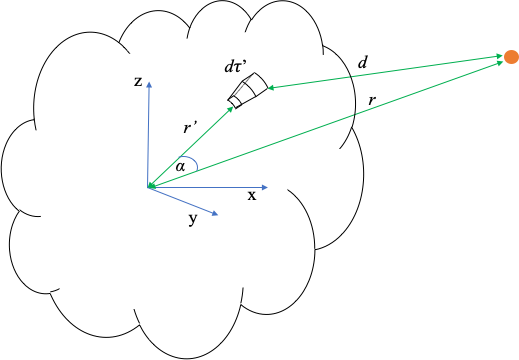
\includegraphics[width=0.45\textwidth]{introduction/continuous_charge.png}}
  \vspace{0pt}
  \caption{foo bar}
  \label{fig:1_1_continuous_charge_distribution}
\end{figure}




\begin{flalign}
    d^2 &= r^2 + (r')^2 - 2rr'\cos \alpha = r^2 \left [ 1 + \left ( \frac{r'}{r} \right)^2 - 2 \left (\frac{r'}{r} \right)\cos \alpha \right]\\
    d &= r \sqrt{1+\epsilon}
    \label{eq:1_1_law_of_cosines}
\end{flalign}

Where,

\begin{flalign}
    \epsilon \equiv \left ( \frac{r'}{r} \right) \left (\frac{r'}{r} - 2 \cos \alpha \right)
\end{flalign}

$\epsilon$ is small far away from charge dist. so can expand $1/d$ binomially

\begin{flalign}
    \frac{1}{d} &= \frac{1}{r}(1+\epsilon)^{-1/2} = \frac{1}{r}\left (1 - \frac{1}{2}\epsilon + \frac{3}{8}\epsilon^2 - ... \right) \\
    \frac{1}{d} &= \frac{1}{r} \sum_{n=0}^{\infty} \left(\frac{r'}{r} \right)^n P_n(\cos \alpha)
\end{flalign}

So can write multipole expansion in terms of legendre polynomials coefficients
exactly in 3D,

\begin{flalign}
    V(\mathbf{r}) = \frac{1}{4 \pi \epsilon_0}\sum_{n=0}^{\infty}\frac{1}{r^{n+1}}\int (r')^nP_n(\cos \alpha)\rho(\mathbf{r'}) d \tau'
\end{flalign}

Again from \cite{Greengard:1987:Yale},

For discrete distributions of $N$ charges $q_i$ this goes to,

\begin{flalign}
    V(\mathbf{r}) = \frac{1}{4 \pi \epsilon_0}\sum_{i=1}^N\sum_{n=0}^{\infty}\frac{(r')^n q_i}{r^{n+1}}P_n(\cos \alpha)
\end{flalign}

Addition theorem for Legendre polynomials,

\begin{flalign}
    P_n(\cos \gamma) = \sum_{m=-n}^n Y_n^{-m}(\alpha, \beta) Y_n^m(\theta, \phi)
\end{flalign}

where two points P and Q with sph. coords. $(r, \theta, \phi)$ and $(\rho, \alpha, \beta)$
$\gamma$ is angle subtended between them,

From addition theorem, Multipole expansion goes to,

\begin{flalign}
    V(\mathbf{r}) &= \frac{1}{4 \pi \epsilon_0}\sum_{i=1}^N\sum_{n=0}^{\infty}\frac{(r')^n q_i}{r^{n+1}}P_n(\cos \alpha)\\
    & = \frac{1}{4 \pi \epsilon_0}\sum_{i=1}^N\sum_{n=0}^{\infty}\sum_{m=-n}^n \frac{(r')^n q_i Y_n^{-m}(\alpha_i, \beta_i) }{r^{n+1}}Y_n^m(\theta, \phi)\\
    & = \sum_{i=1}^N\sum_{n=0}^{\infty}\sum_{m=-n}^n\frac{M_n^m}{r^{n+1}} \cdot Y_n^m(\theta, \phi)
\end{flalign}

This is an exact expansion, can be truncated as reqiured for tunable precision.



\begin{figure}[!h]
    \centering
    {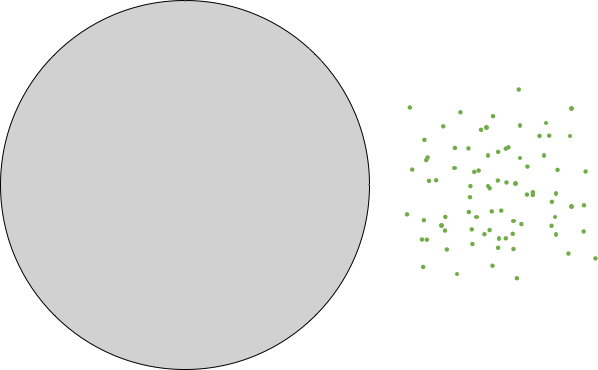
\includegraphics[width=0.45\textwidth]{introduction/multipole_expansion.png}}
    \hfill
  {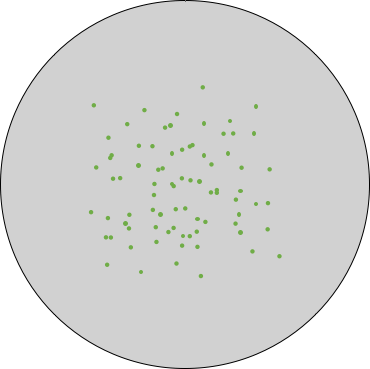
\includegraphics[width=0.28\textwidth]{introduction/local_expansion.png}}
  \vspace{0pt}
  \caption{foo bar}
  \label{fig:1_1_multipole_local_expansions}
\end{figure}



\textbf{Notes from \cite{Griffiths:2017:CUP}}

page 152 develops the multipole expansion for the potential of an arbitrary
charge distribution in 3D.


$\mathbf{r}$ - vector from centre of expansion at charge distribution to the point
of evaluation, $d$ - the  distance from volume element $d\tau'$ to the point of
evaluation, $\rho(\mathbf{r}')$ - charge density, $\mathbf{r}'$ - the vector
from the centre of expansion to the volume element. $alpha$ is the angle between
$r$ and $r'$.


If instead expansion taken with centre at targets, at distance from sources, Can
rewrite as Local Expansion.

\begin{flalign}
    V(\mathbf{r}) = \frac{1}{4 \pi \epsilon_0} \sum_{i=1}^N \sum_{j=0}^{\infty} \sum_{k=-j}^j L_j^k \cdot  Y_j^k(\theta, \phi) \cdot r^j
\end{flalign}

Where the coefficients of the local expansion can be derived from the coefficients
of the the multipole expansion.

Analytic expressions for shifting multipole and local expansions explained. Should
probably specify shift operators in appendix for completeness...
These shifts are exact.

\hspace{10pt}

\subsection{Algorithm structure}

\textbf{Notes from \cite{Ying:2004:JCP}}

FMM makes use of these representations in a recursive algorithm. computational
domain is a box containing all particles, sources and targets. Hierarchically
partitioned into a tree structure, called Octree in 3D. With each level $l$ of the
tree partitioned into $8^l$ geometric boxes. For each box, the potential induced
by it's source densities is represented by a multipole expansion centered around
the box, while the potential induced by the sources from non-adjacent boxes is
encoded in a local expansion.

Number of expansion terms $p$ is chosen for a prescribed relative error $\epsilon$,
using $p=\log_c \epsilon$ where $c=\frac{4-\sqrt{3}}{\sqrt{3}}$ in 3D (numerically optimal?).
The trucation error has rigorous bounds.

The availability of analytic translations enable the $\mathcal{O}(n)$ algorithm.
In particular the following translations; M2M, L2L, M2L.

Two basic steps of FMM using tree structure.

\begin{enumerate}
    \item \textit{Upward Pass} The tree is traversed, post-order. S2M at leaves
    - compute multipole expansion of leaf sources at leaf node. Shift multipole
    expansion to parent node, and sum together.
    \item \textit{Downward Pass} The tree is traversed pre-order. The local expansion
    for each box is the sum of two parts: (1) the L2L transformation collects the local
    expansion of B's parent (compressing the information for boxes non-adjacent to B's parent)
    (2) the M2l translation, for each multipole expansion of boxes which are the children of
    the neighbors of B's parent but not adjacent to B itself.At the end of the
    Downward Pass, the `far' interaction which is evaluated
    using the local expansion at this box (L2T operation) at each target particle.
    Combined with the `near' interaction by direct computation of potential over all
    source points in near field (within the box itself, and it's direct neighbors).
\end{enumerate}


\begin{figure}[!h]
    \centering
    {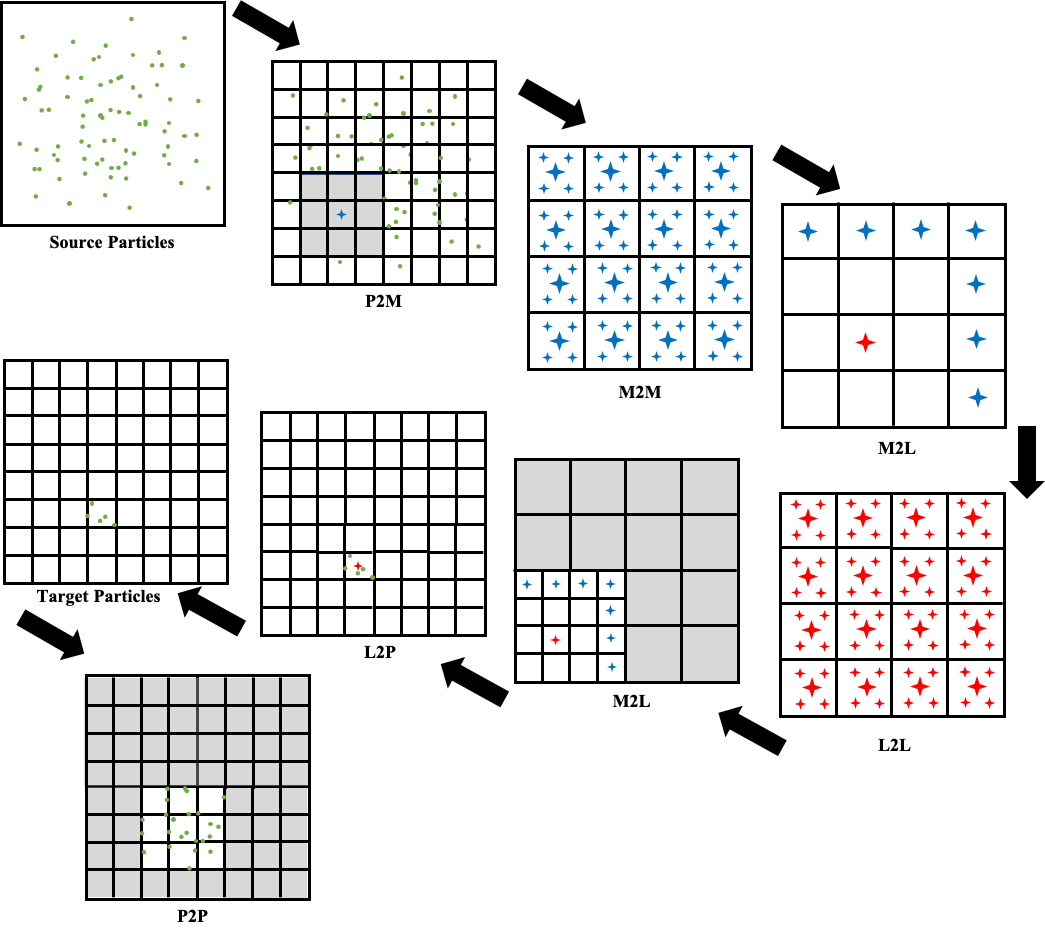
\includegraphics[width=\textwidth]{introduction/main_loop.png}}
  \vspace{0pt}
  \caption{foo bar}
  \label{fig:1_1_main_loop}
\end{figure}


\subsection{Analysis}

Begin with $O(N\log(N))$ algorithm variant; here post order traversal (from
coarsest to finest level), compute multipole expansion for each box at each level,
this has the $Np^2$ bound, at finest level assume $O(1)$ number of particles, so
direct computation with nearest neighbour particles leads to $O(N)$ bound.

Full analysis defer to \cite{Greengard:1987:Yale}. Enough to understand that the
translation operators are what lead to the $\mathcal{O}(n)$ complexity. Beginning
with upward pass, at leaf level each particle contributes to one expansion so
S2M of the order $Np^2$ - $p^2$ is the order of operations for the multipole
expansion, can see this from the equation. M2M/L2L/M2L shifts require $p^4$
operations, so all are bounded by $O(Np^4)$ (consider last level), precise bound
dictated by number of boxes in interaction list. Evaluating the $p^th$ degree
local expansions at each target particle (L2T) bounded by $O(Np^2)$, small constant
$\kappa$ particles enforced at leaf level leads to $O(\kappa N)$ complexity for
direct calculations at leaf level. We see that the whole algorithm is bounded by
$O(N)$.

\hspace{10pt}
